\documentclass{beamer}

\usepackage[utf8]{inputenc}
\usepackage{default}
\usepackage{xcolor}

\title{All colours are beautiful}
\institute{MetaMeute}

\usetheme{Madrid}

\begin{document}

\setbeamertemplate{headline}{}
\beamertemplatenavigationsymbolsempty
\setbeamercolor{frametitle}{bg=black}
\setbeamercolor{section in head/foot}{bg=black}
\setbeamercolor{footlinecolor}{fg=white,bg=black}
\setbeamertemplate{footline}{}

\setbeamertemplate{itemize item}{\color{black}$\blacktriangleright$}
\setbeamertemplate{itemize subitem}{\color{black}$\blacktriangleright$}

\newcommand{\myitem}[2]{\item[\textcolor{gray}{#1}] \textcolor{black}{\emph{#2}}}

{
\setbeamercolor{background canvas}{bg=black, fg=white}
\setbeamertemplate{footline}{}

\begin{frame}
 \centering
 
\includegraphics[width=10cm,keepaspectratio=true]{./title_because_gnxtr_sucks_at_beamer.png}
\end{frame}


\begin{frame}
 \centering
 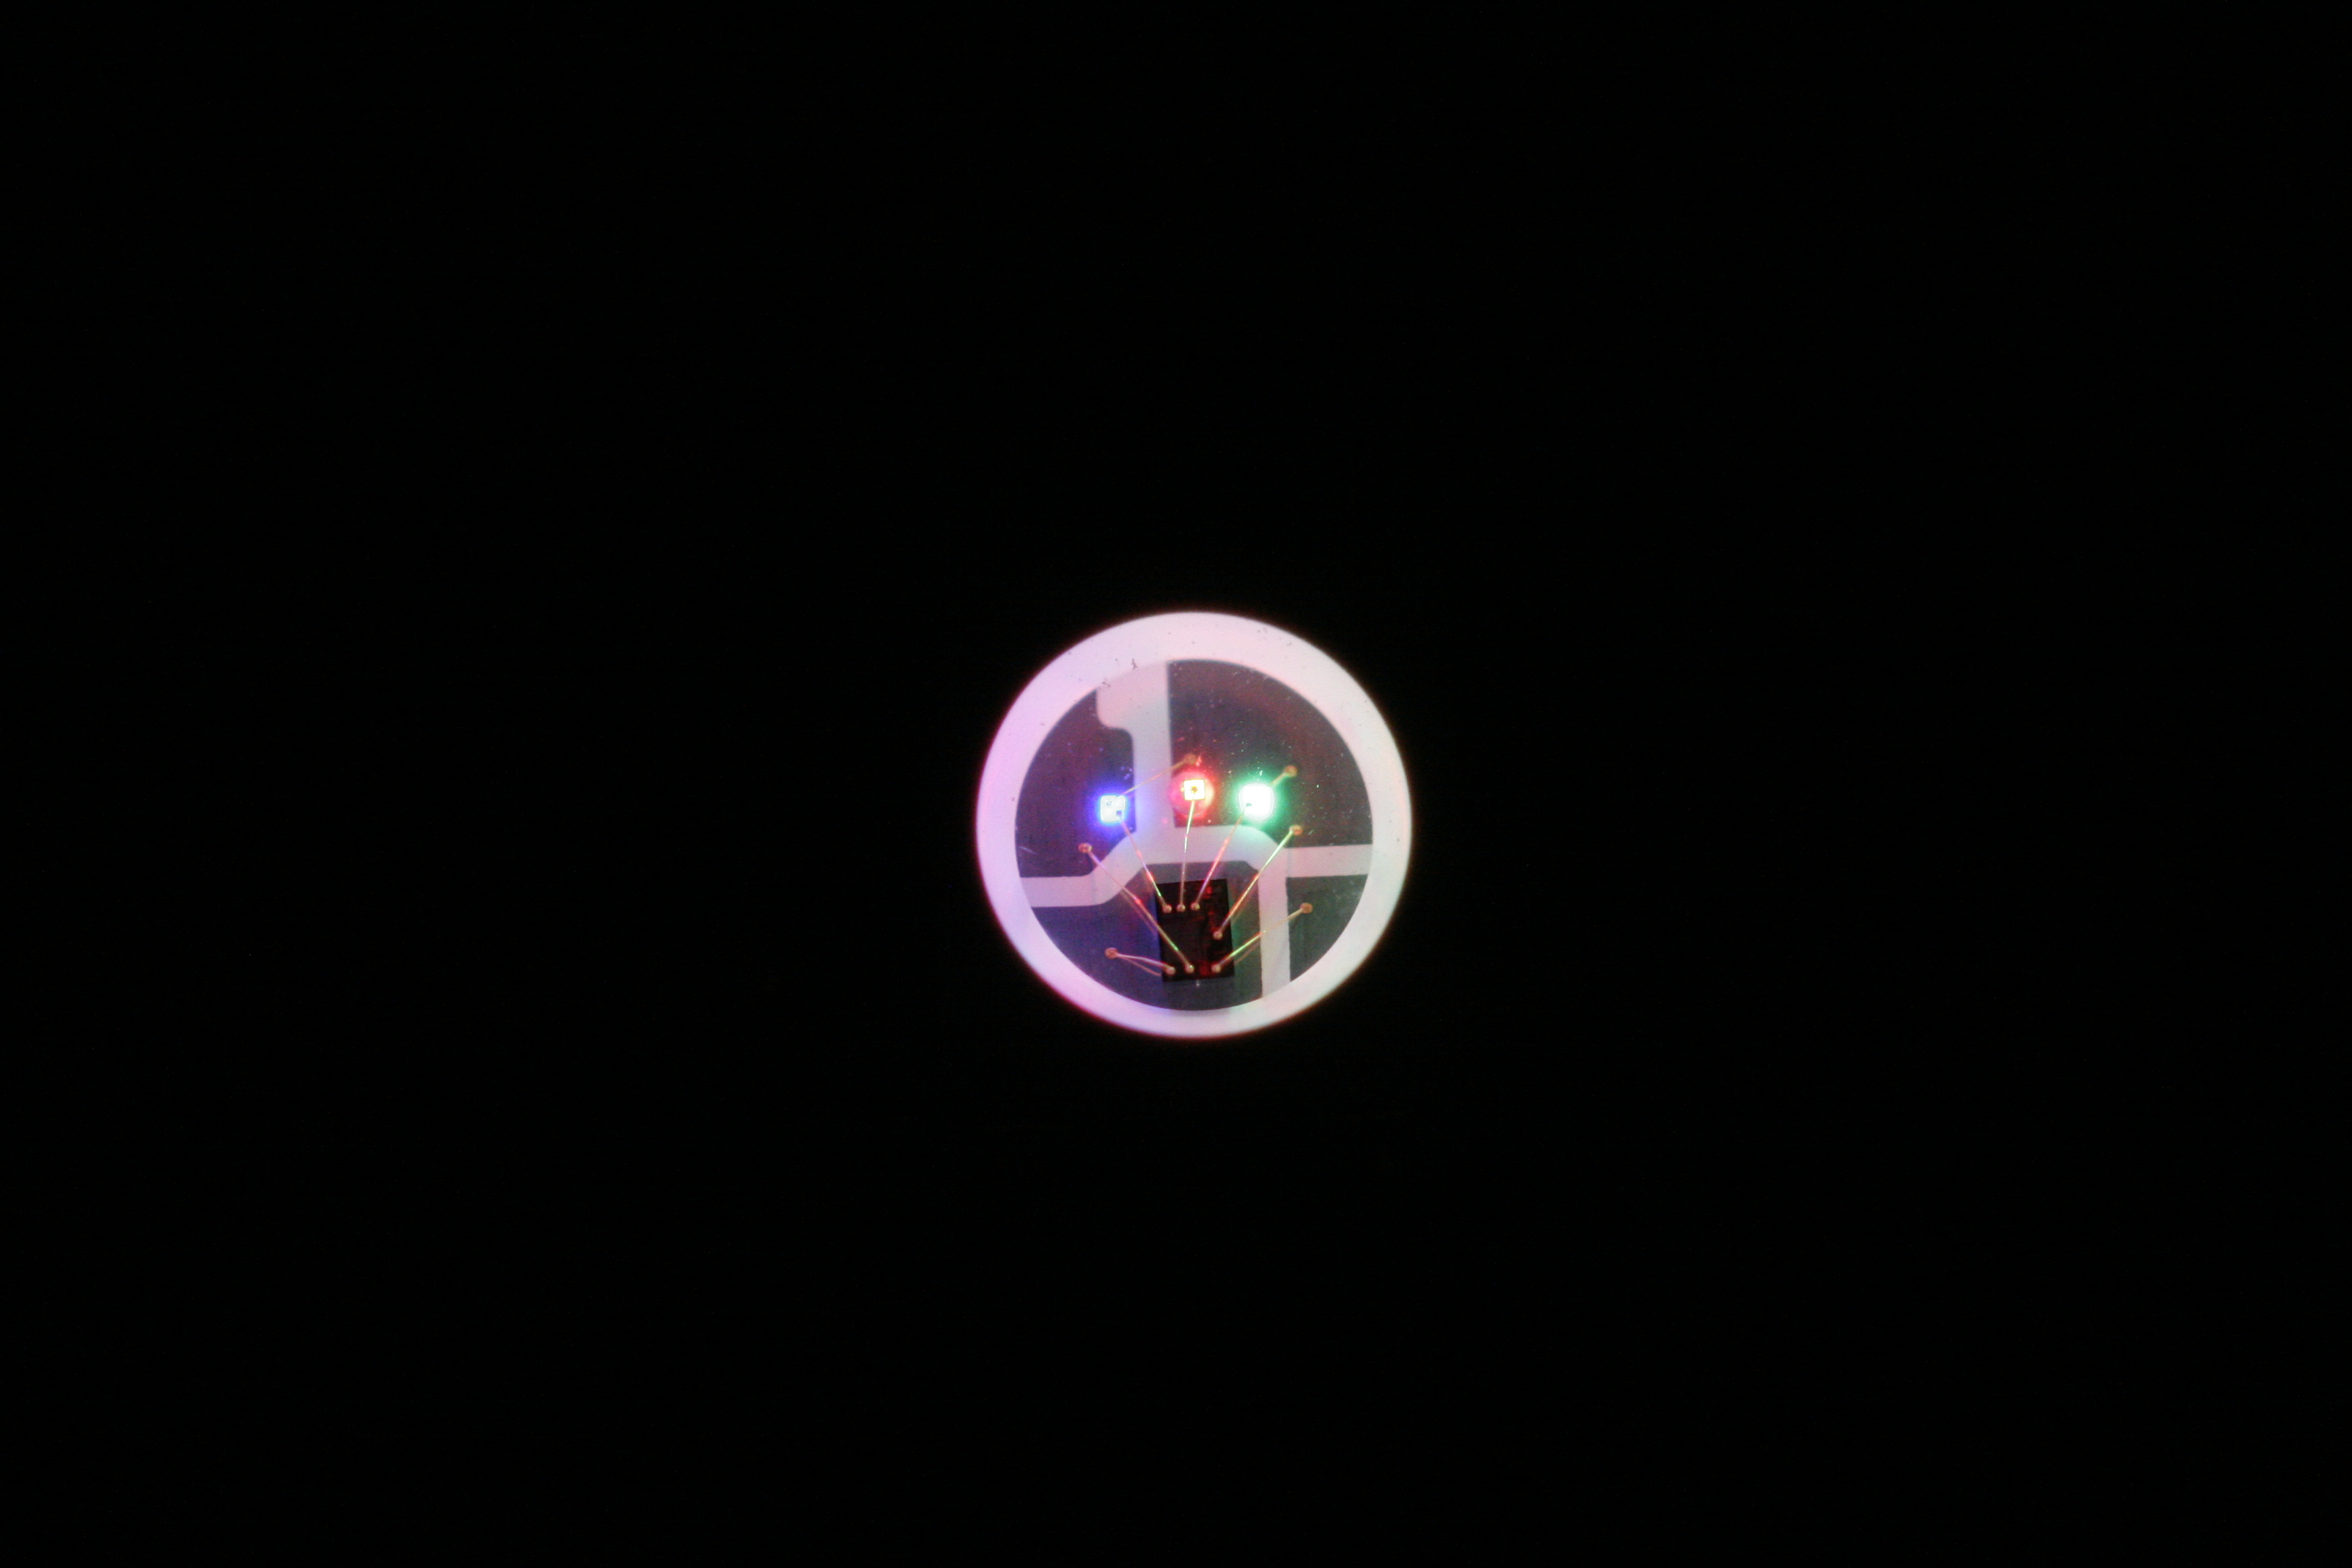
\includegraphics[width=10cm,keepaspectratio=true]{./img/_MG_4513.JPG}
\end{frame}

}
\section{Bezugsquellendiskussion}
\begin{frame}{Bezugsquellendiskussion}
\begin{itemize}
 \item Angebote einholen
 \item Geldtransferkosten (Klassische Überweisung)
 \item Einfuhrumsatzsteuer, Zoll, Freibeträge
 \item Vor der Bestellung: Drei Wege Handshake
\end{itemize}
\end{frame}

\section{Aufbau}
\subsection{Strom}
\begin{frame}{Strom}
\begin{figure}[h]
 \centering
 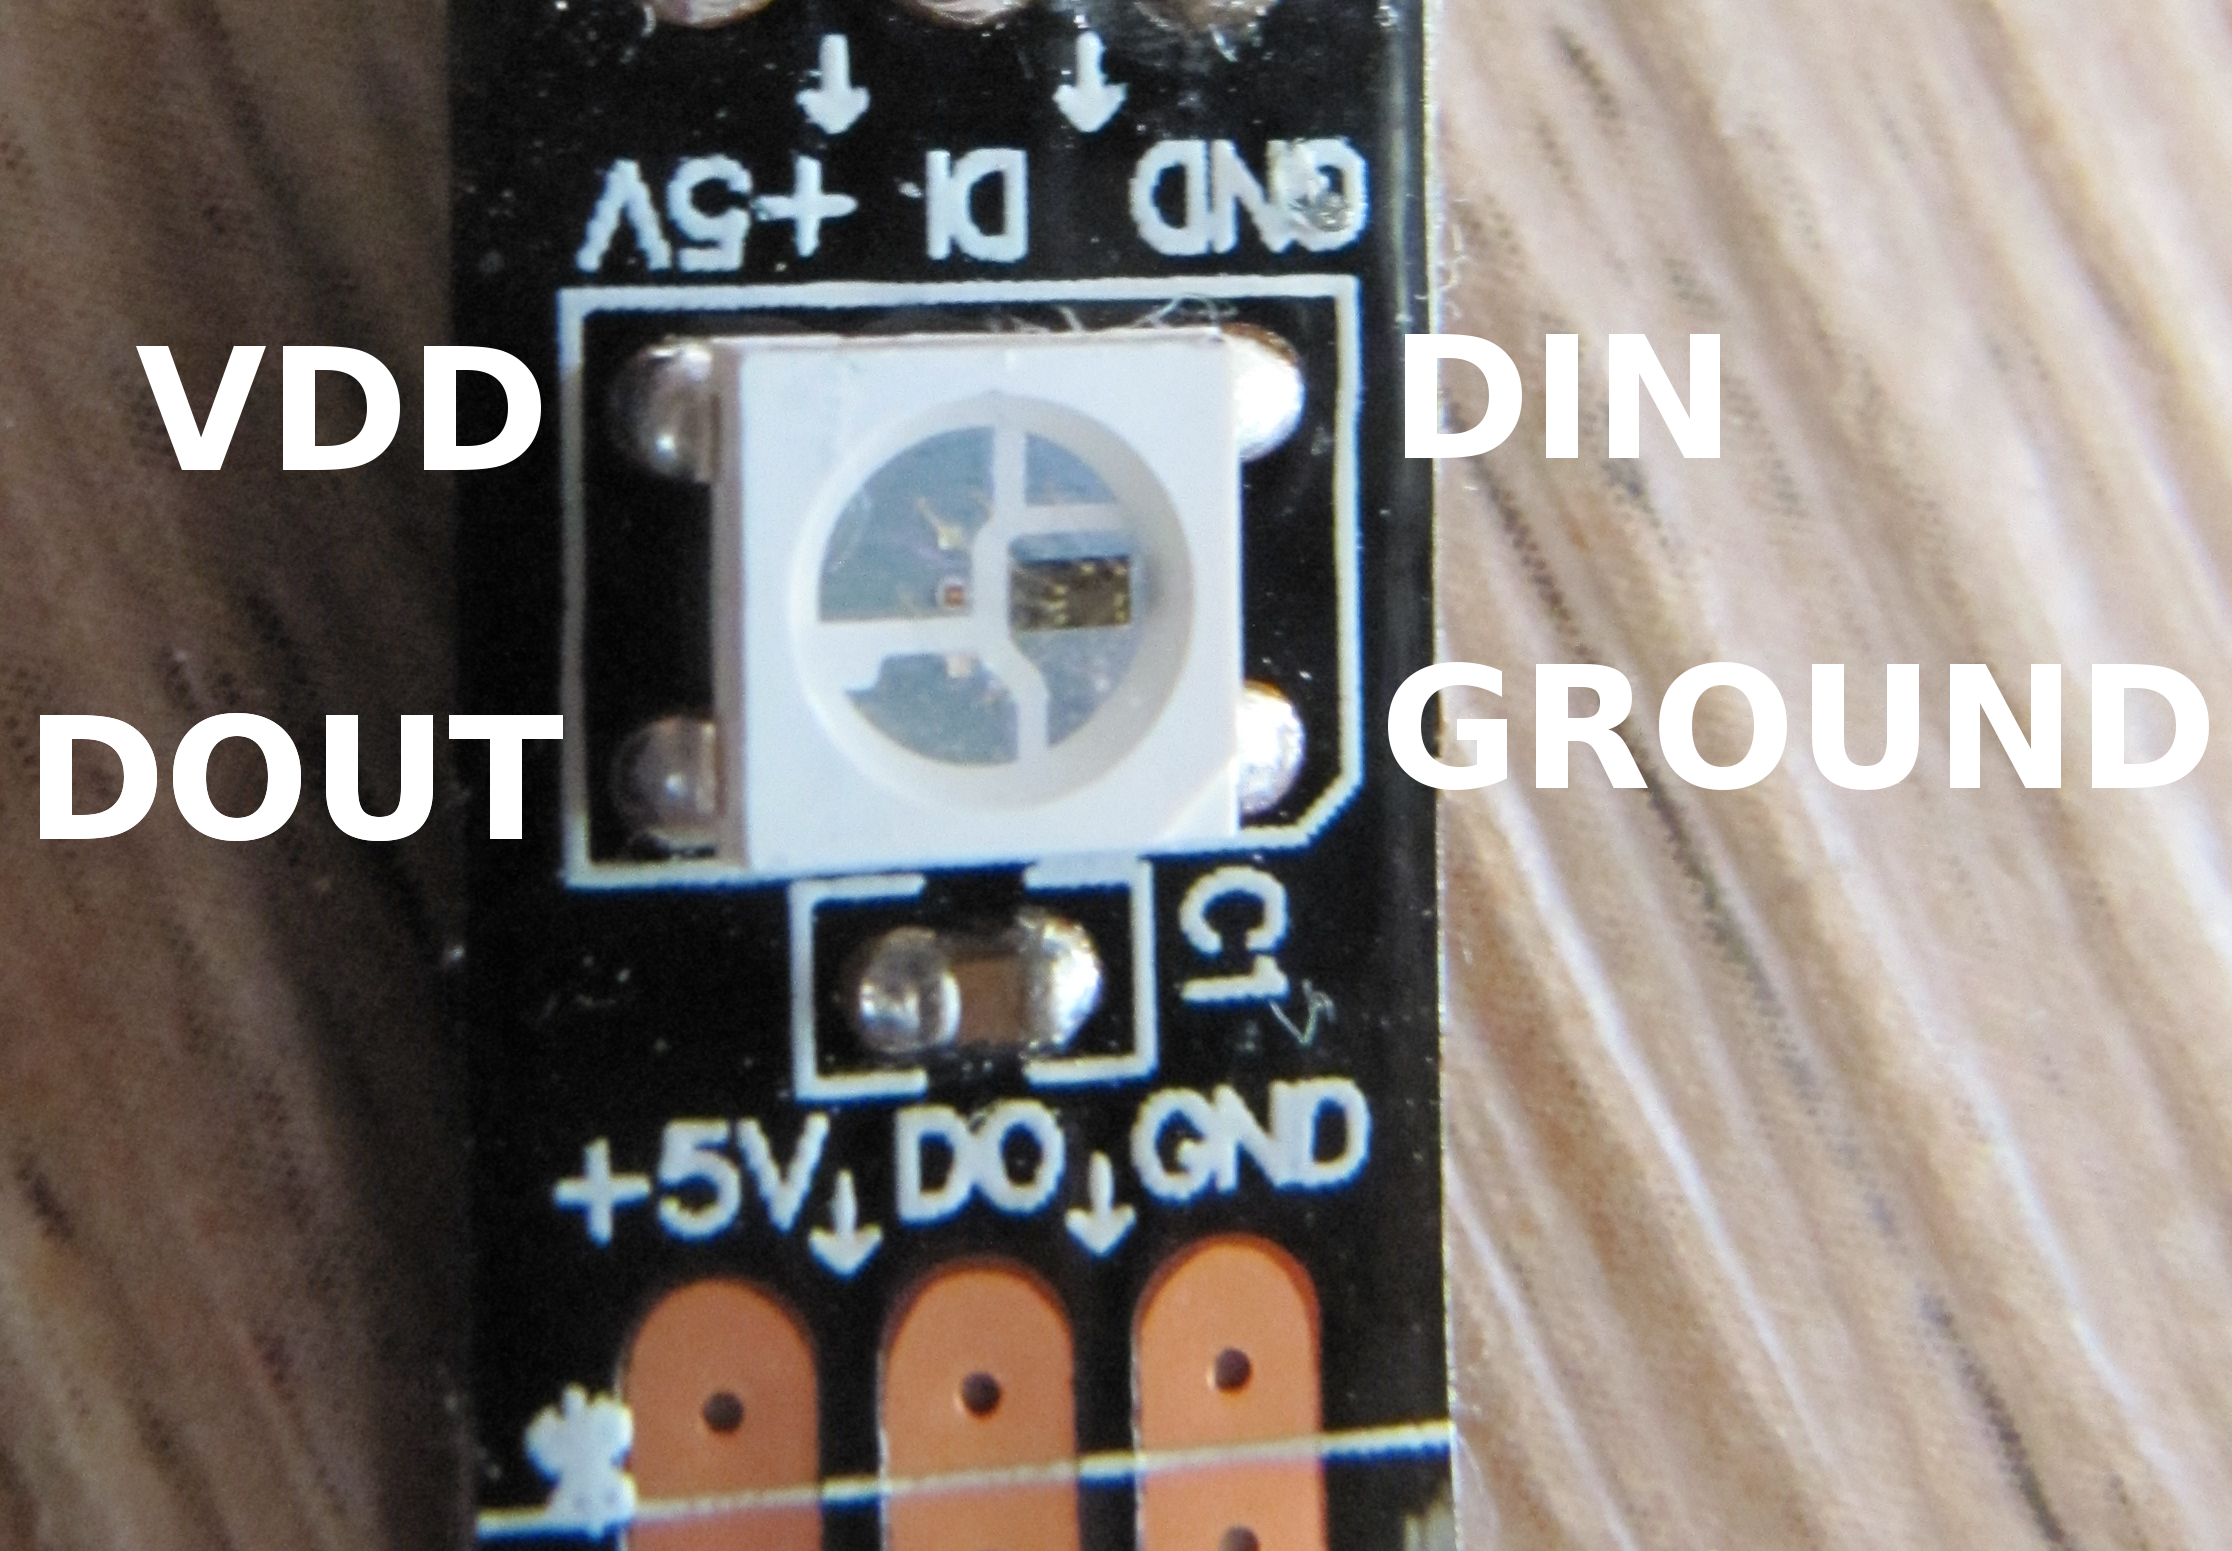
\includegraphics[width=5cm,keepaspectratio=true]{./WS2812B_CloseUp.png}
\end{figure}

\begin{description}
\myitem{Versorgung}{5V}
\myitem{Strom}{20mA}
\myitem{Logic Level}{Low  $<$ 0.3$\cdot$VDD, 0.7$\cdot$VDD $<$ High}
\end{description}

\end{frame}

\subsection{Protokoll}
\begin{frame}{Protokoll}
\begin{center}
 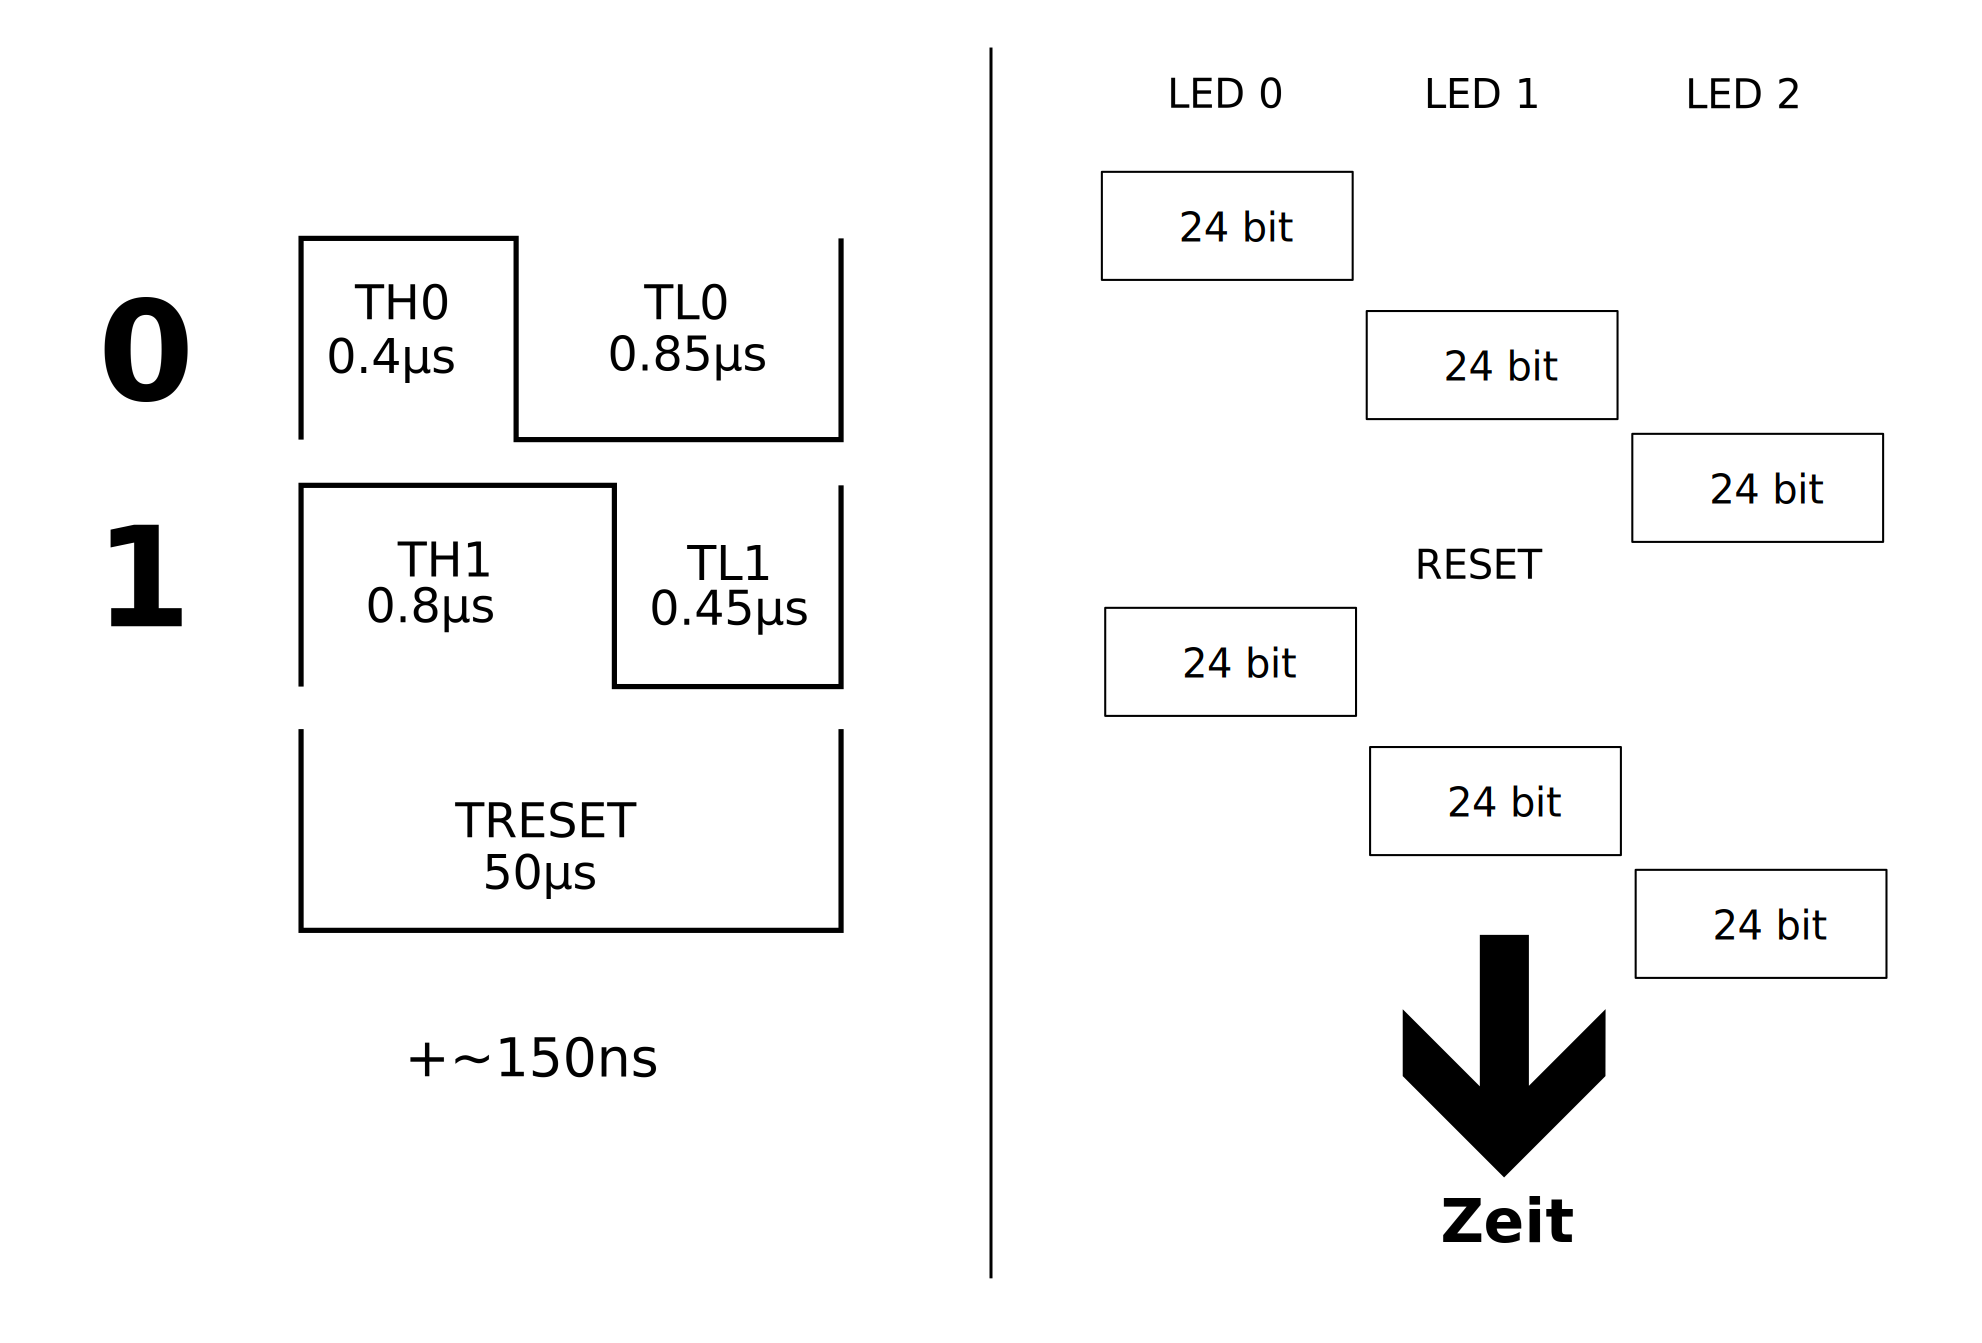
\includegraphics[width=11cm]{protokoll}
\end{center}
\end{frame}

\section{Ansteuerung}
\subsection{Arduino}
\begin{frame}{Arduino}
\begin{figure}[h]
 \centering
 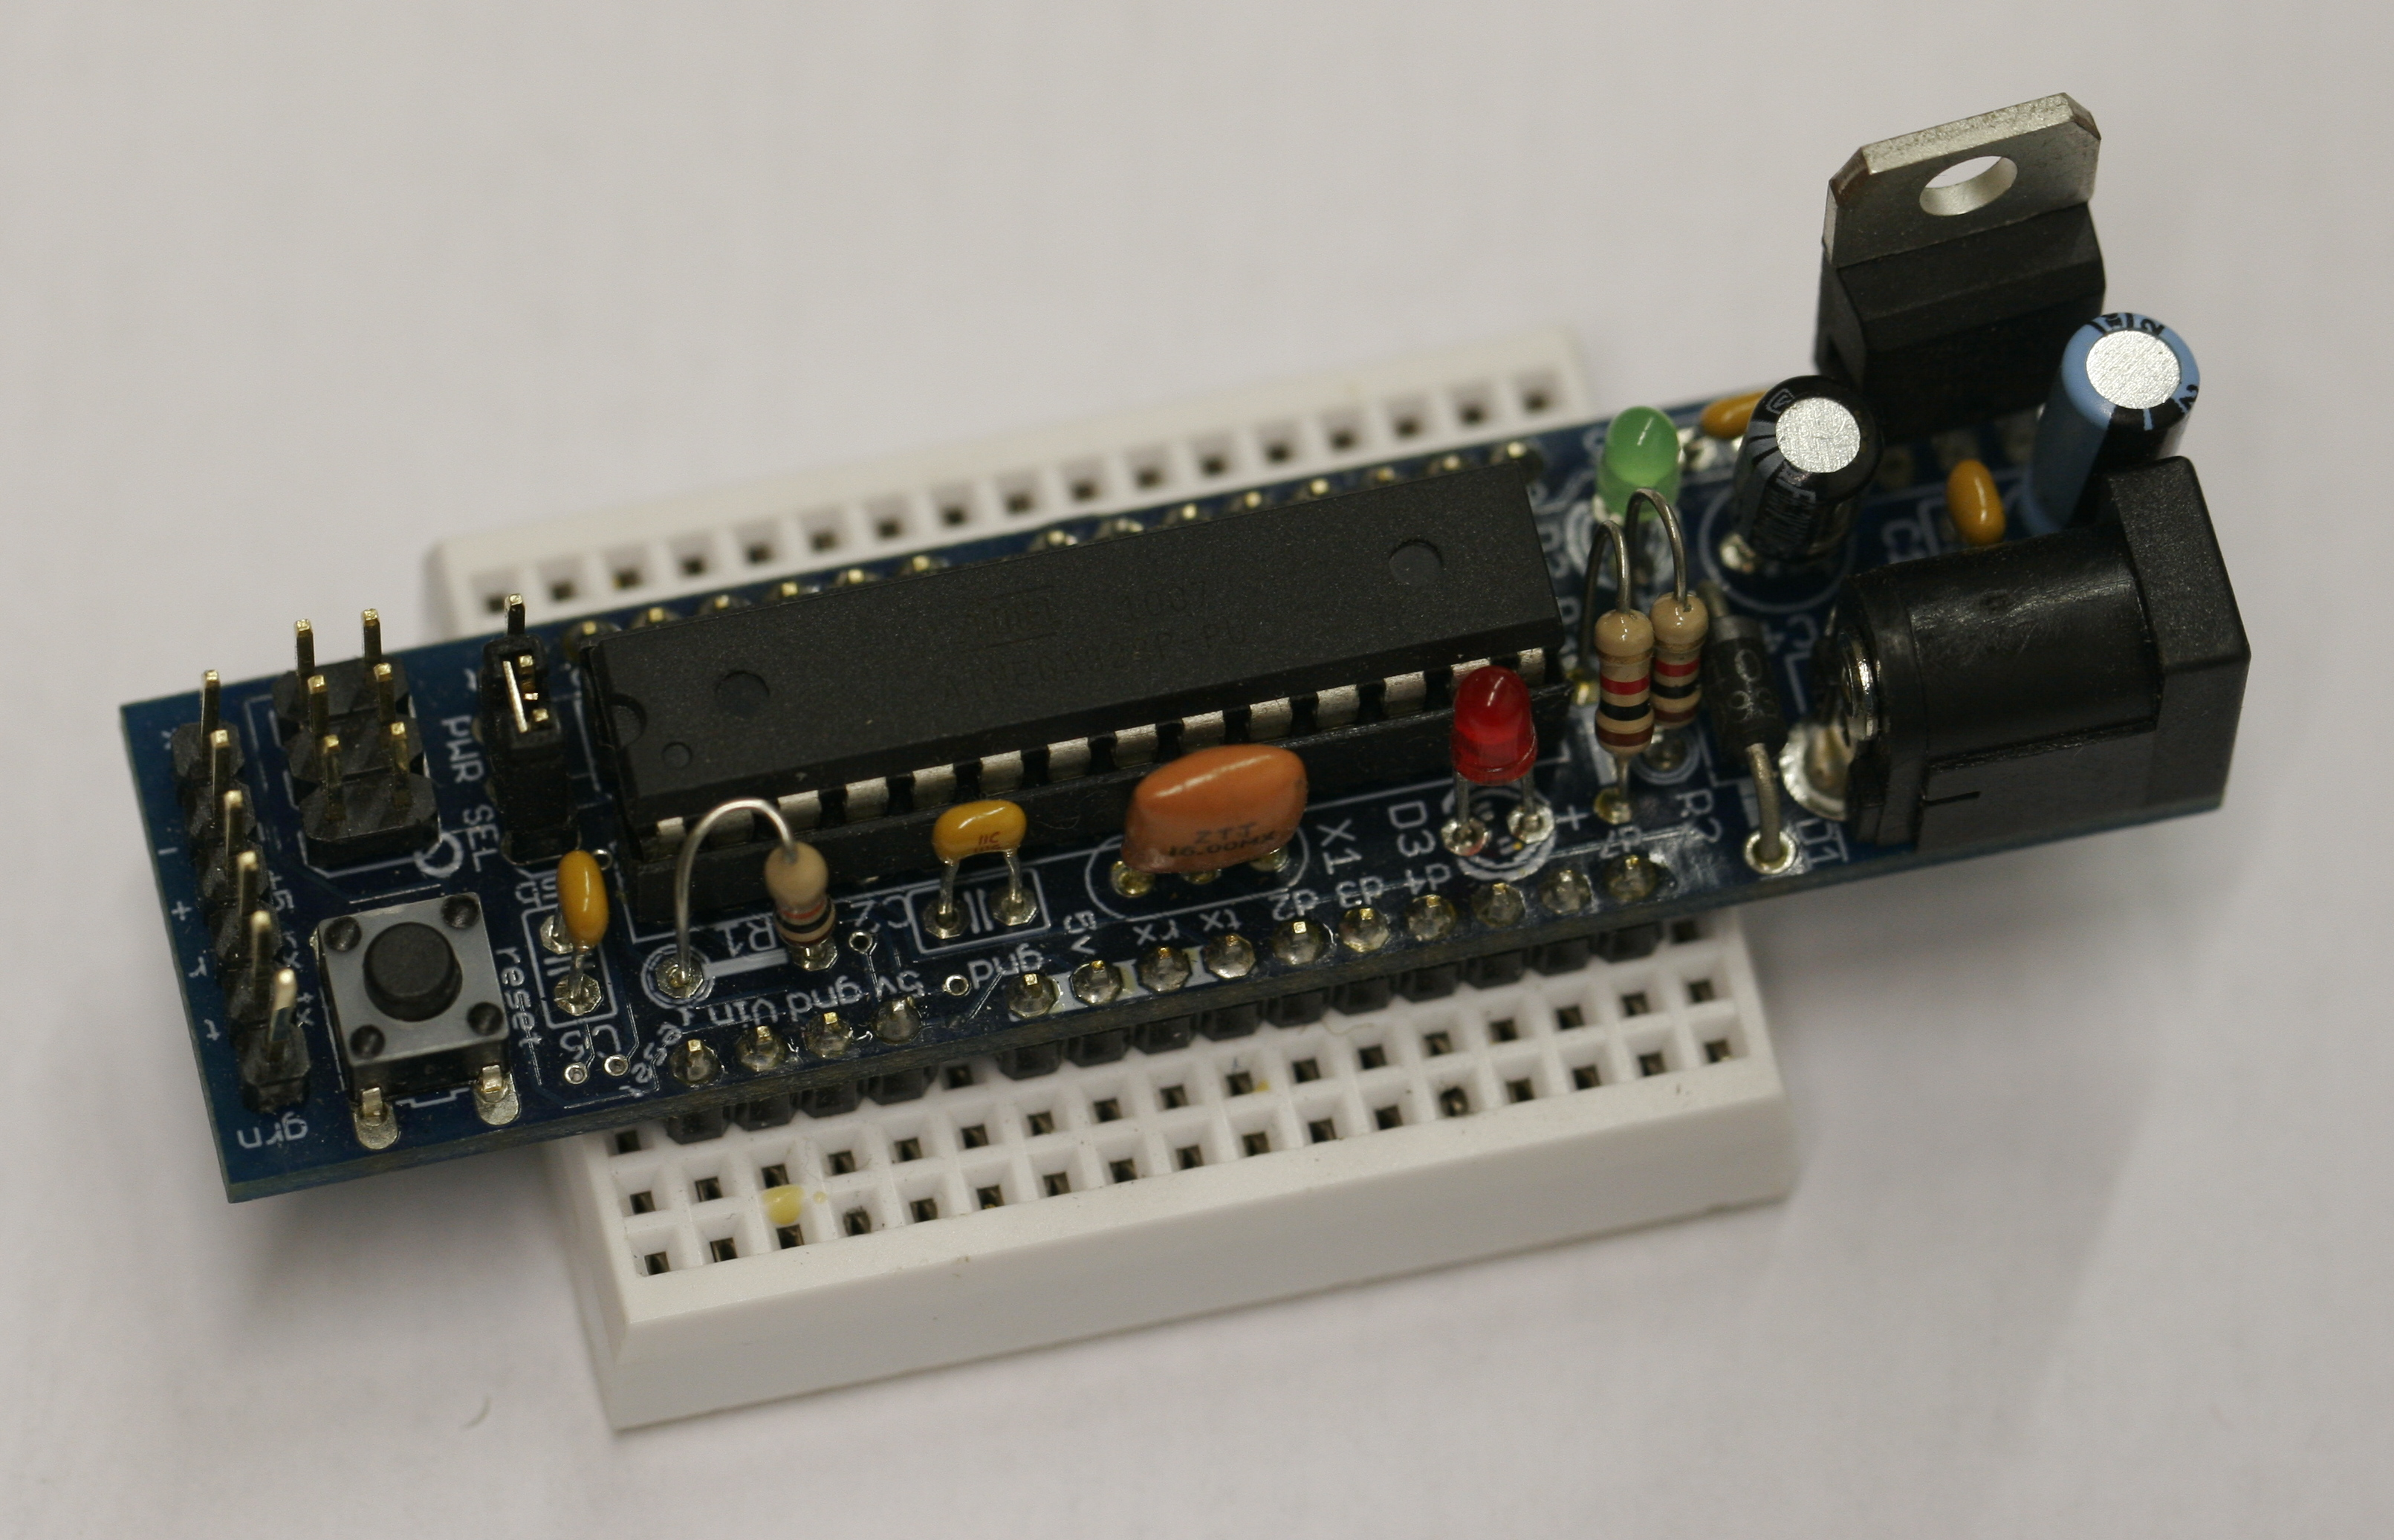
\includegraphics[width=6cm,keepaspectratio=true]{./img/_MG_4522.JPG}
\end{figure}
\begin{itemize}
 \item Anfängerorientiertes I/O Board
 \item Hauptsächlich AVR Chips
 \item Viele Varianten, umfangreiche Libraries

\end{itemize}
\end{frame}

\subsection{FTDI}
\begin{frame}{FTDI}
\begin{figure}[h]
 \centering
 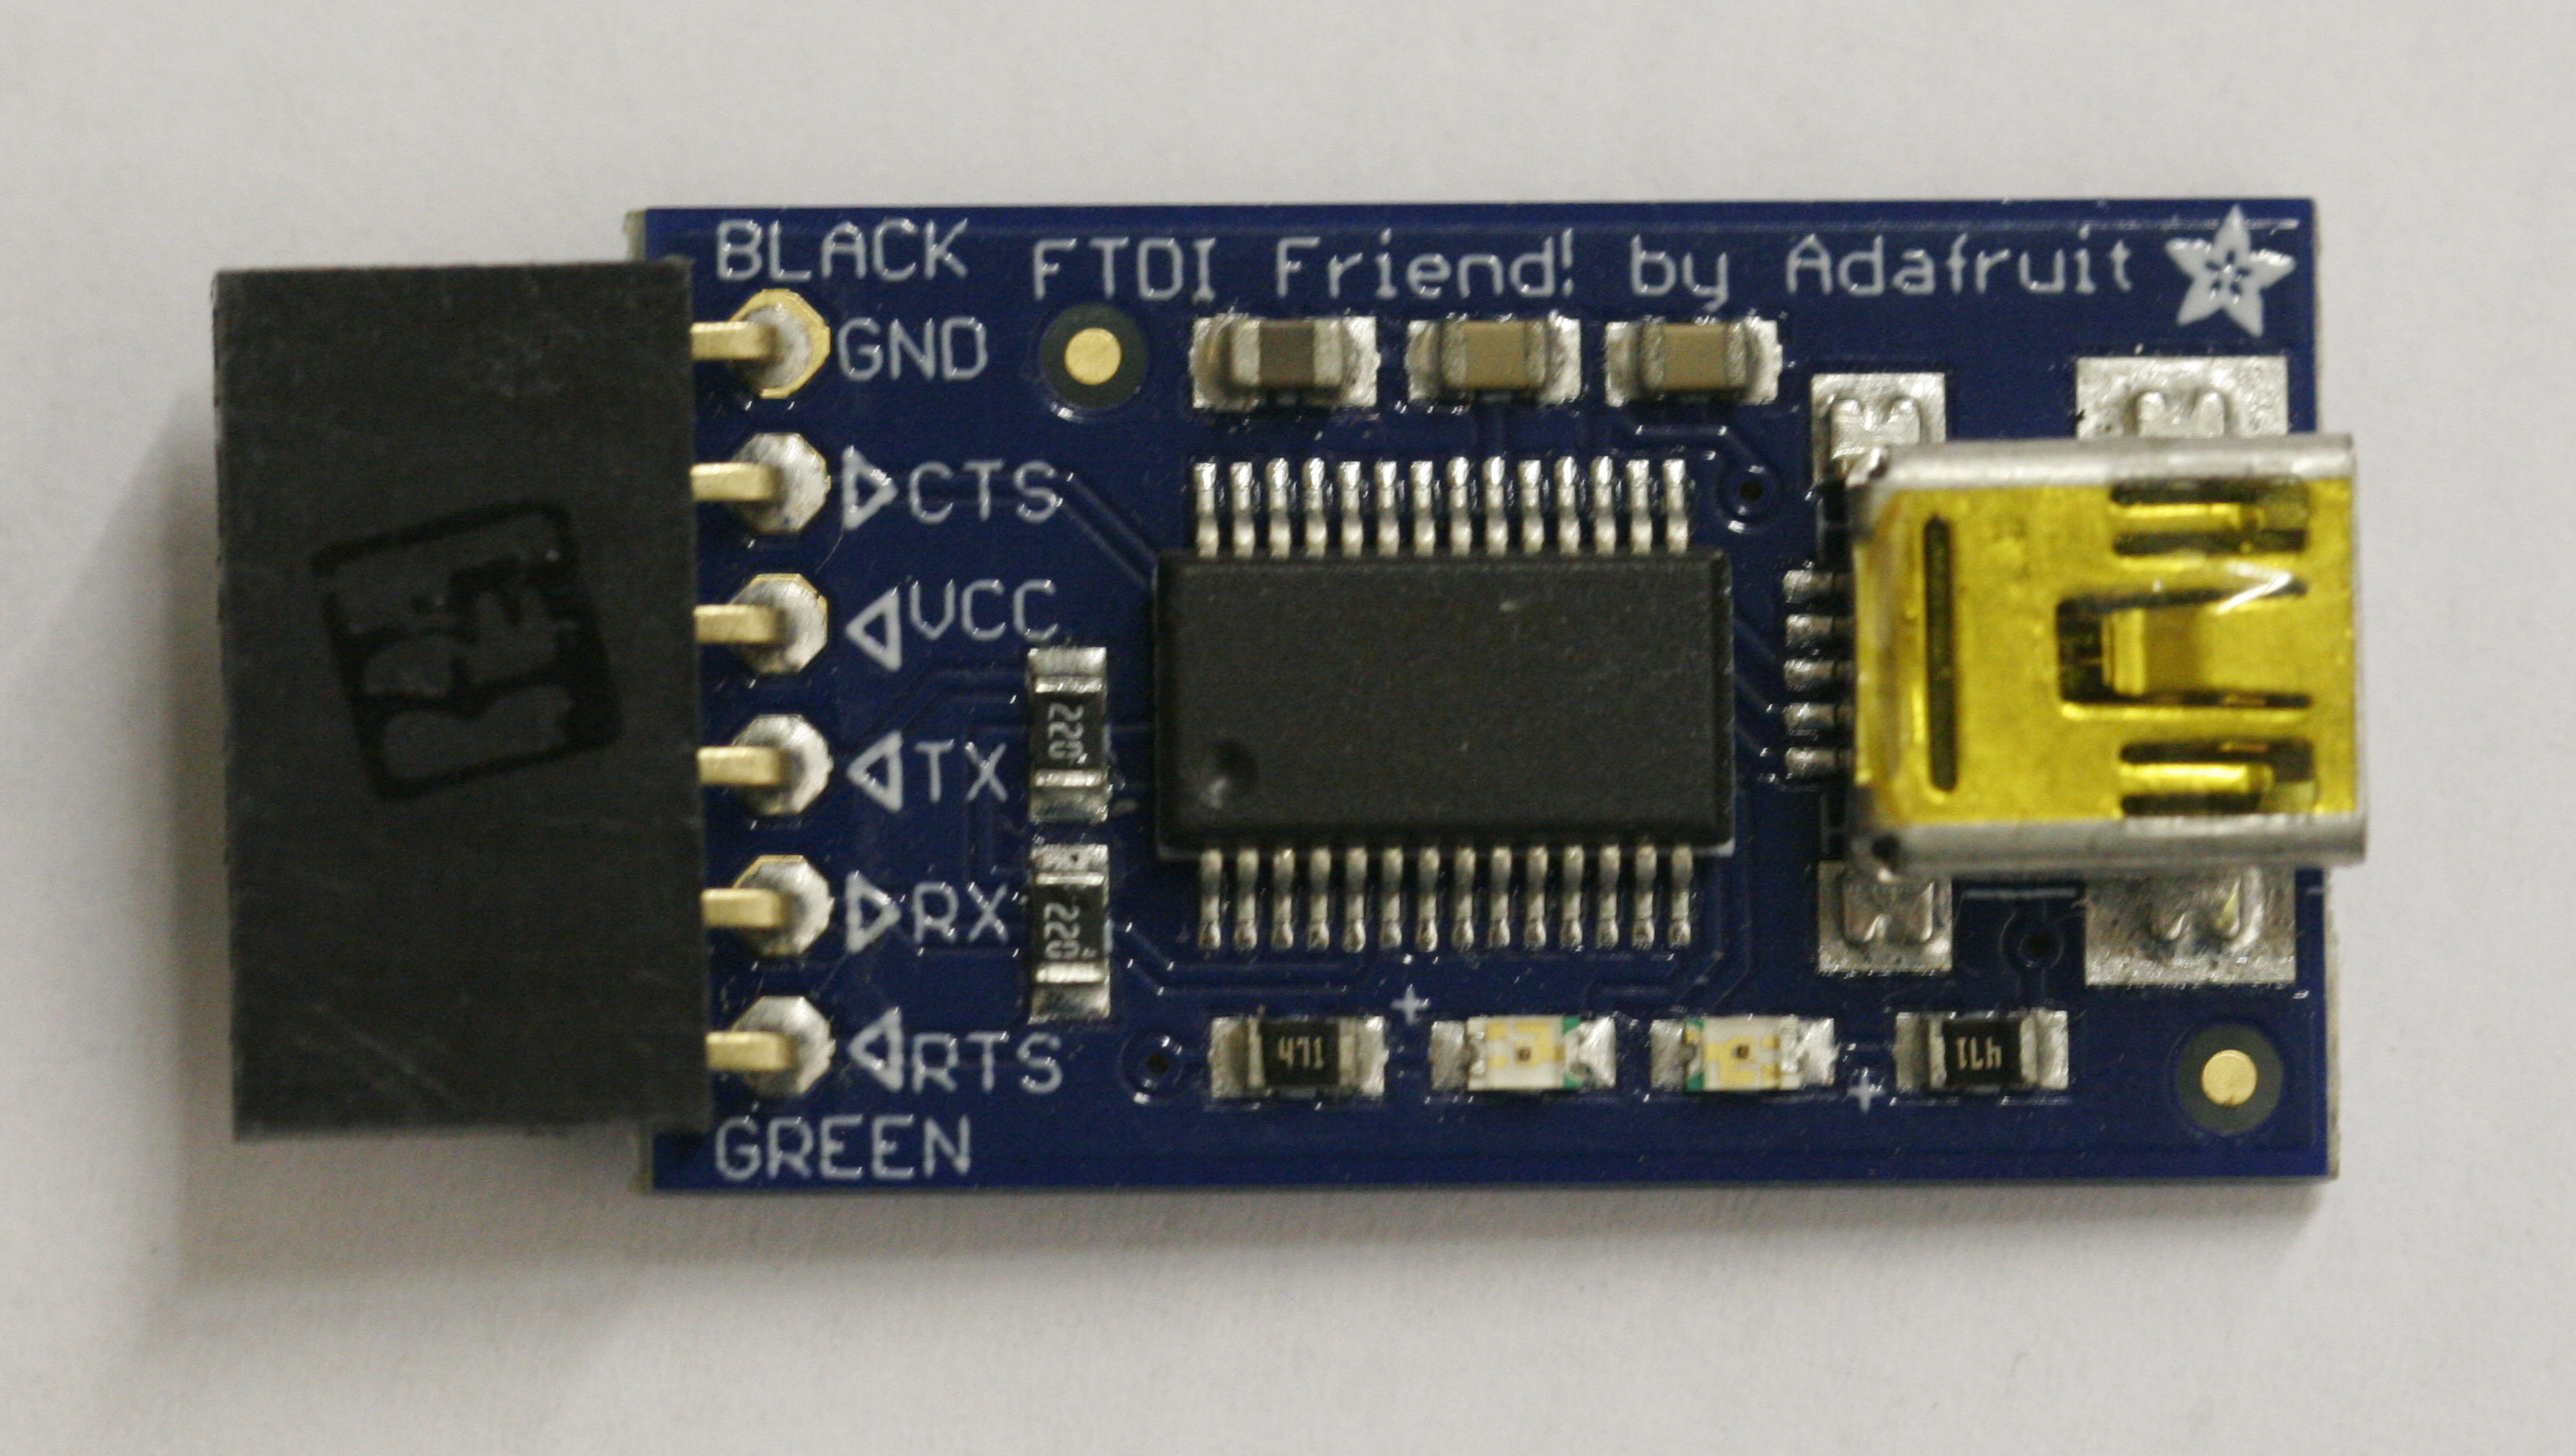
\includegraphics[width=6cm,keepaspectratio=true]{./img/_MG_4517.JPG}
\end{figure}
\begin{itemize}
 \item Seriell to USB Converter
 \item 3V und 5V Logic
 \item Programmierer für Arduinos, AVRs und Stromversorgung
\end{itemize}

\end{frame}


\subsection{VoCore}
\begin{frame}{VoCore}
\begin{figure}[h]
 \centering
 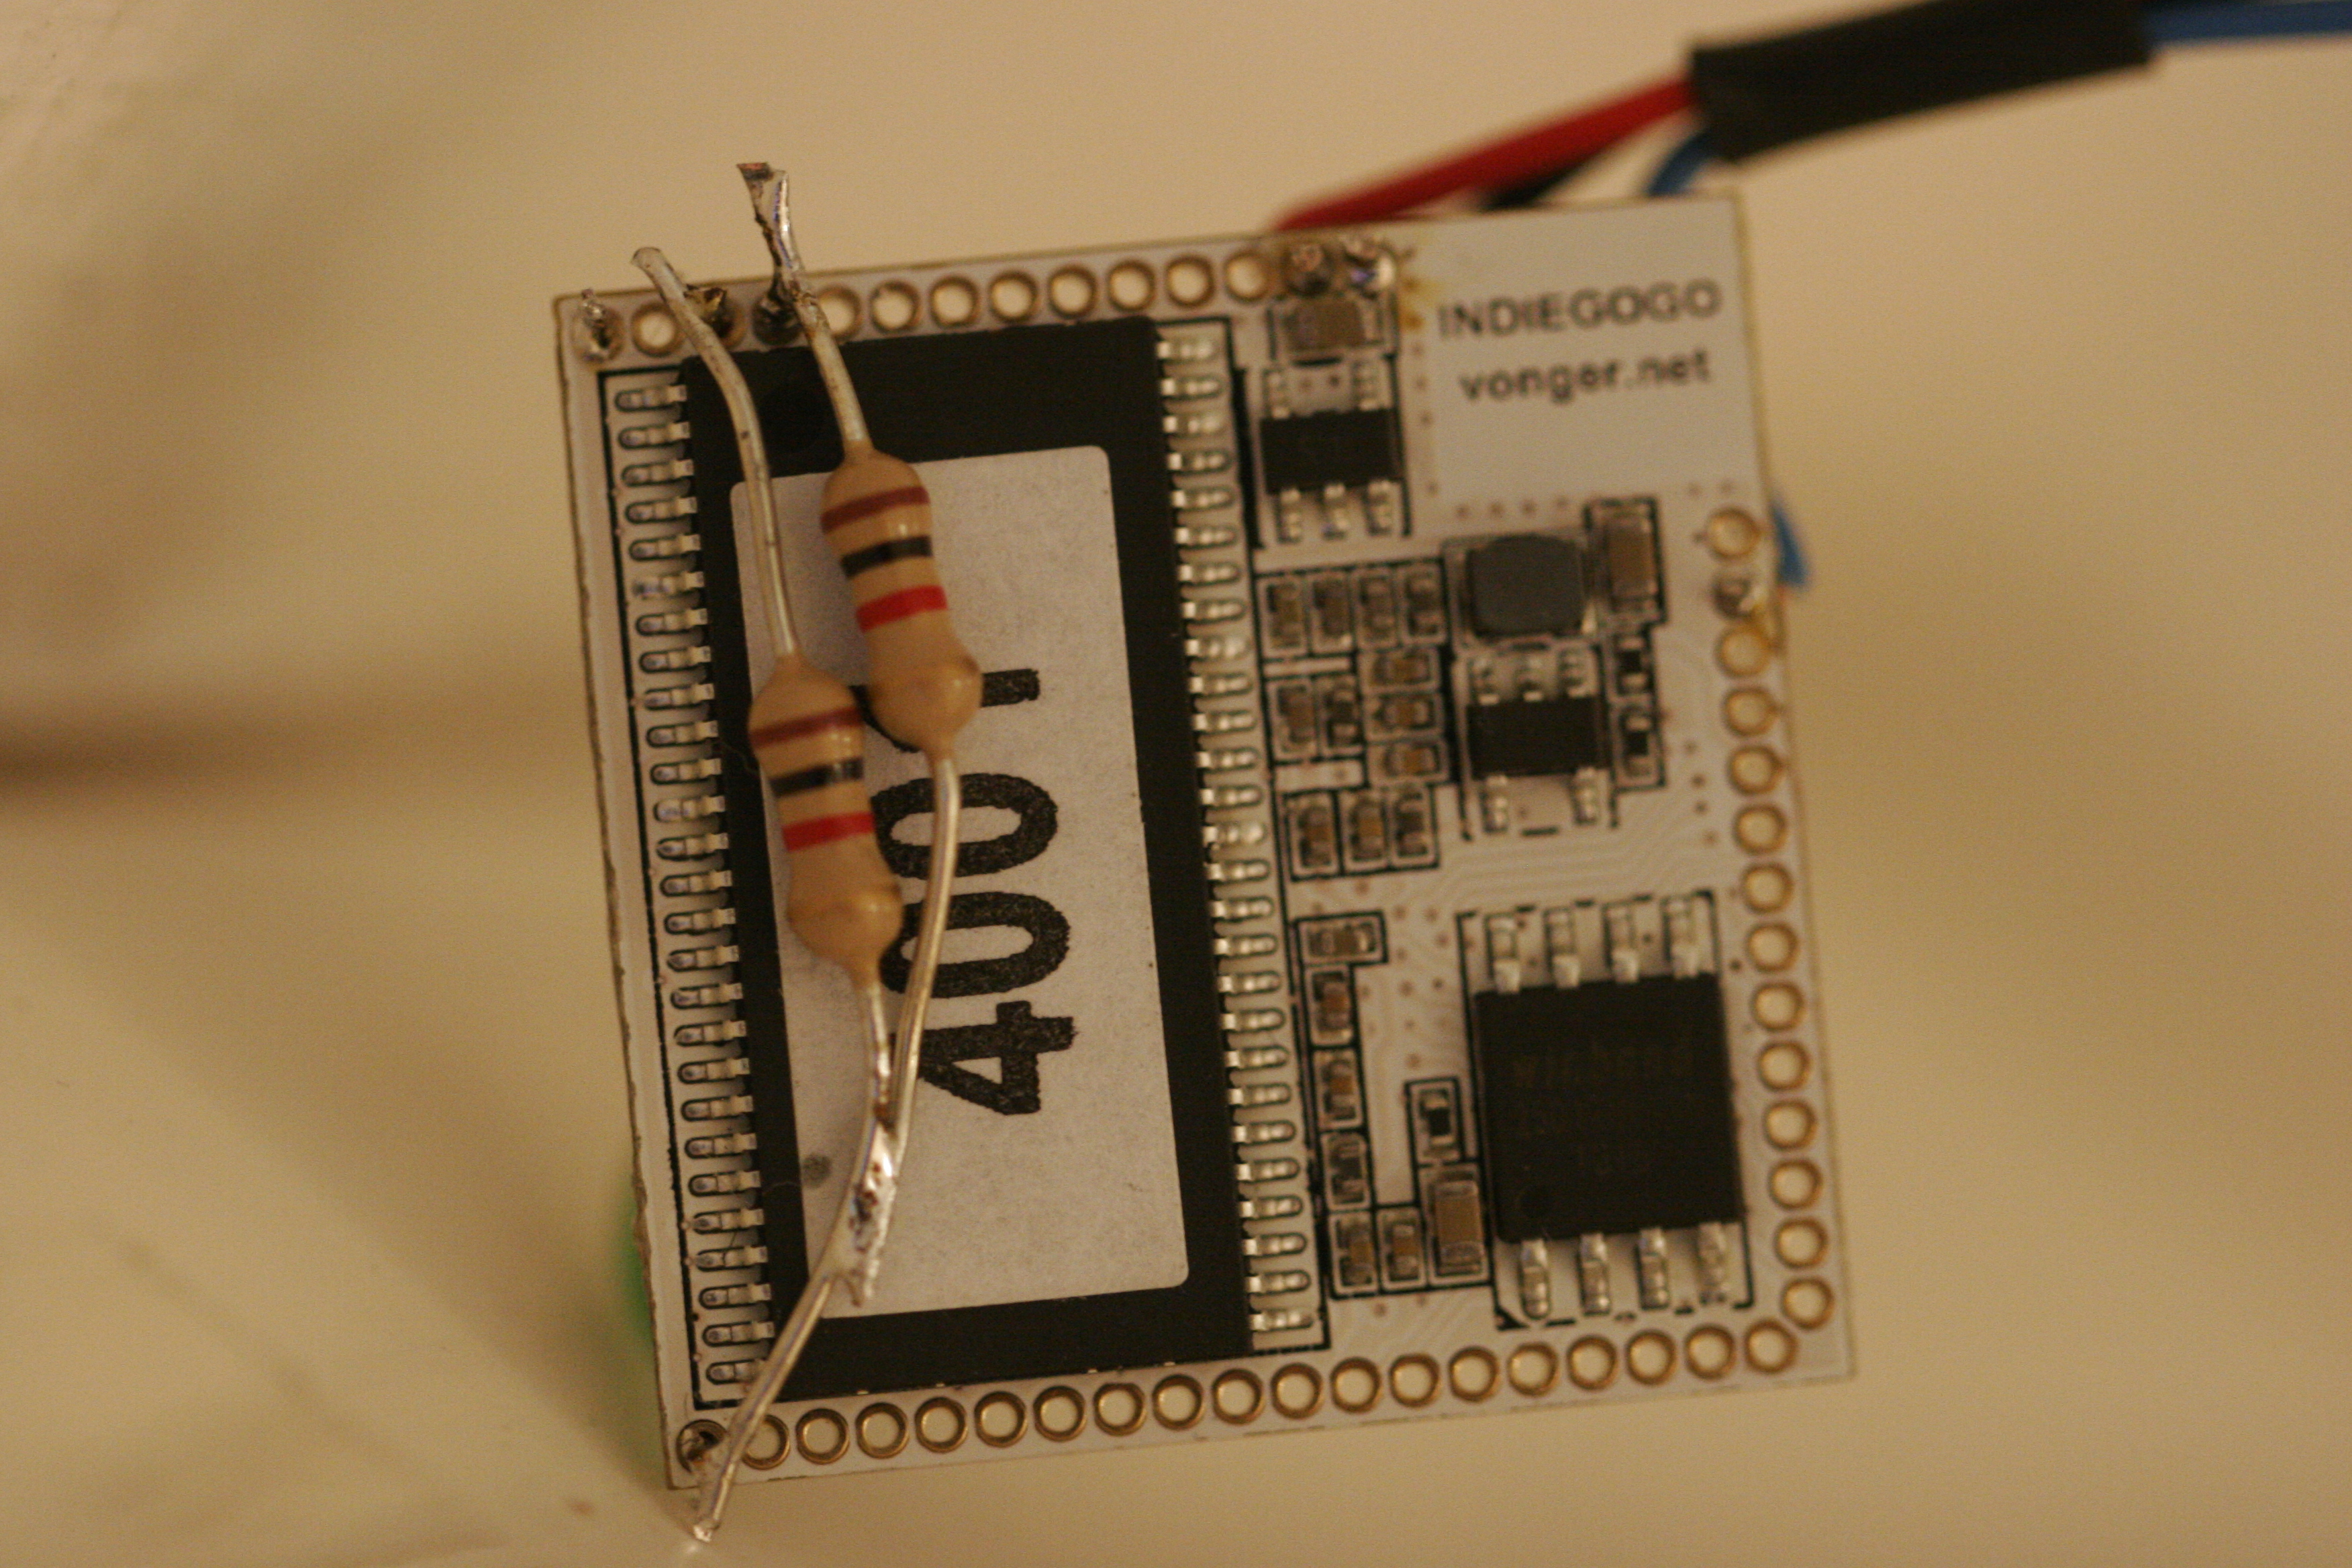
\includegraphics[width=6cm,keepaspectratio=true]{./img/_MG_4492.JPG}
\end{figure}
\begin{itemize}
 \item 2.5x2.5cm SoC (360MHz, 32MB) mit OpenWrt
 \item Günstig, mit Wifi 802.11n, Ethernet 10/100MHz
 \item Unterstützt USB, UART, SPI, I2C, Ethernet mit 28 GPIOs
\end{itemize}
\end{frame}

\section{Projekte}
\subsection{Freifunk-Logo}
\begin{frame}{Freifunk-Logo}
 \centering
 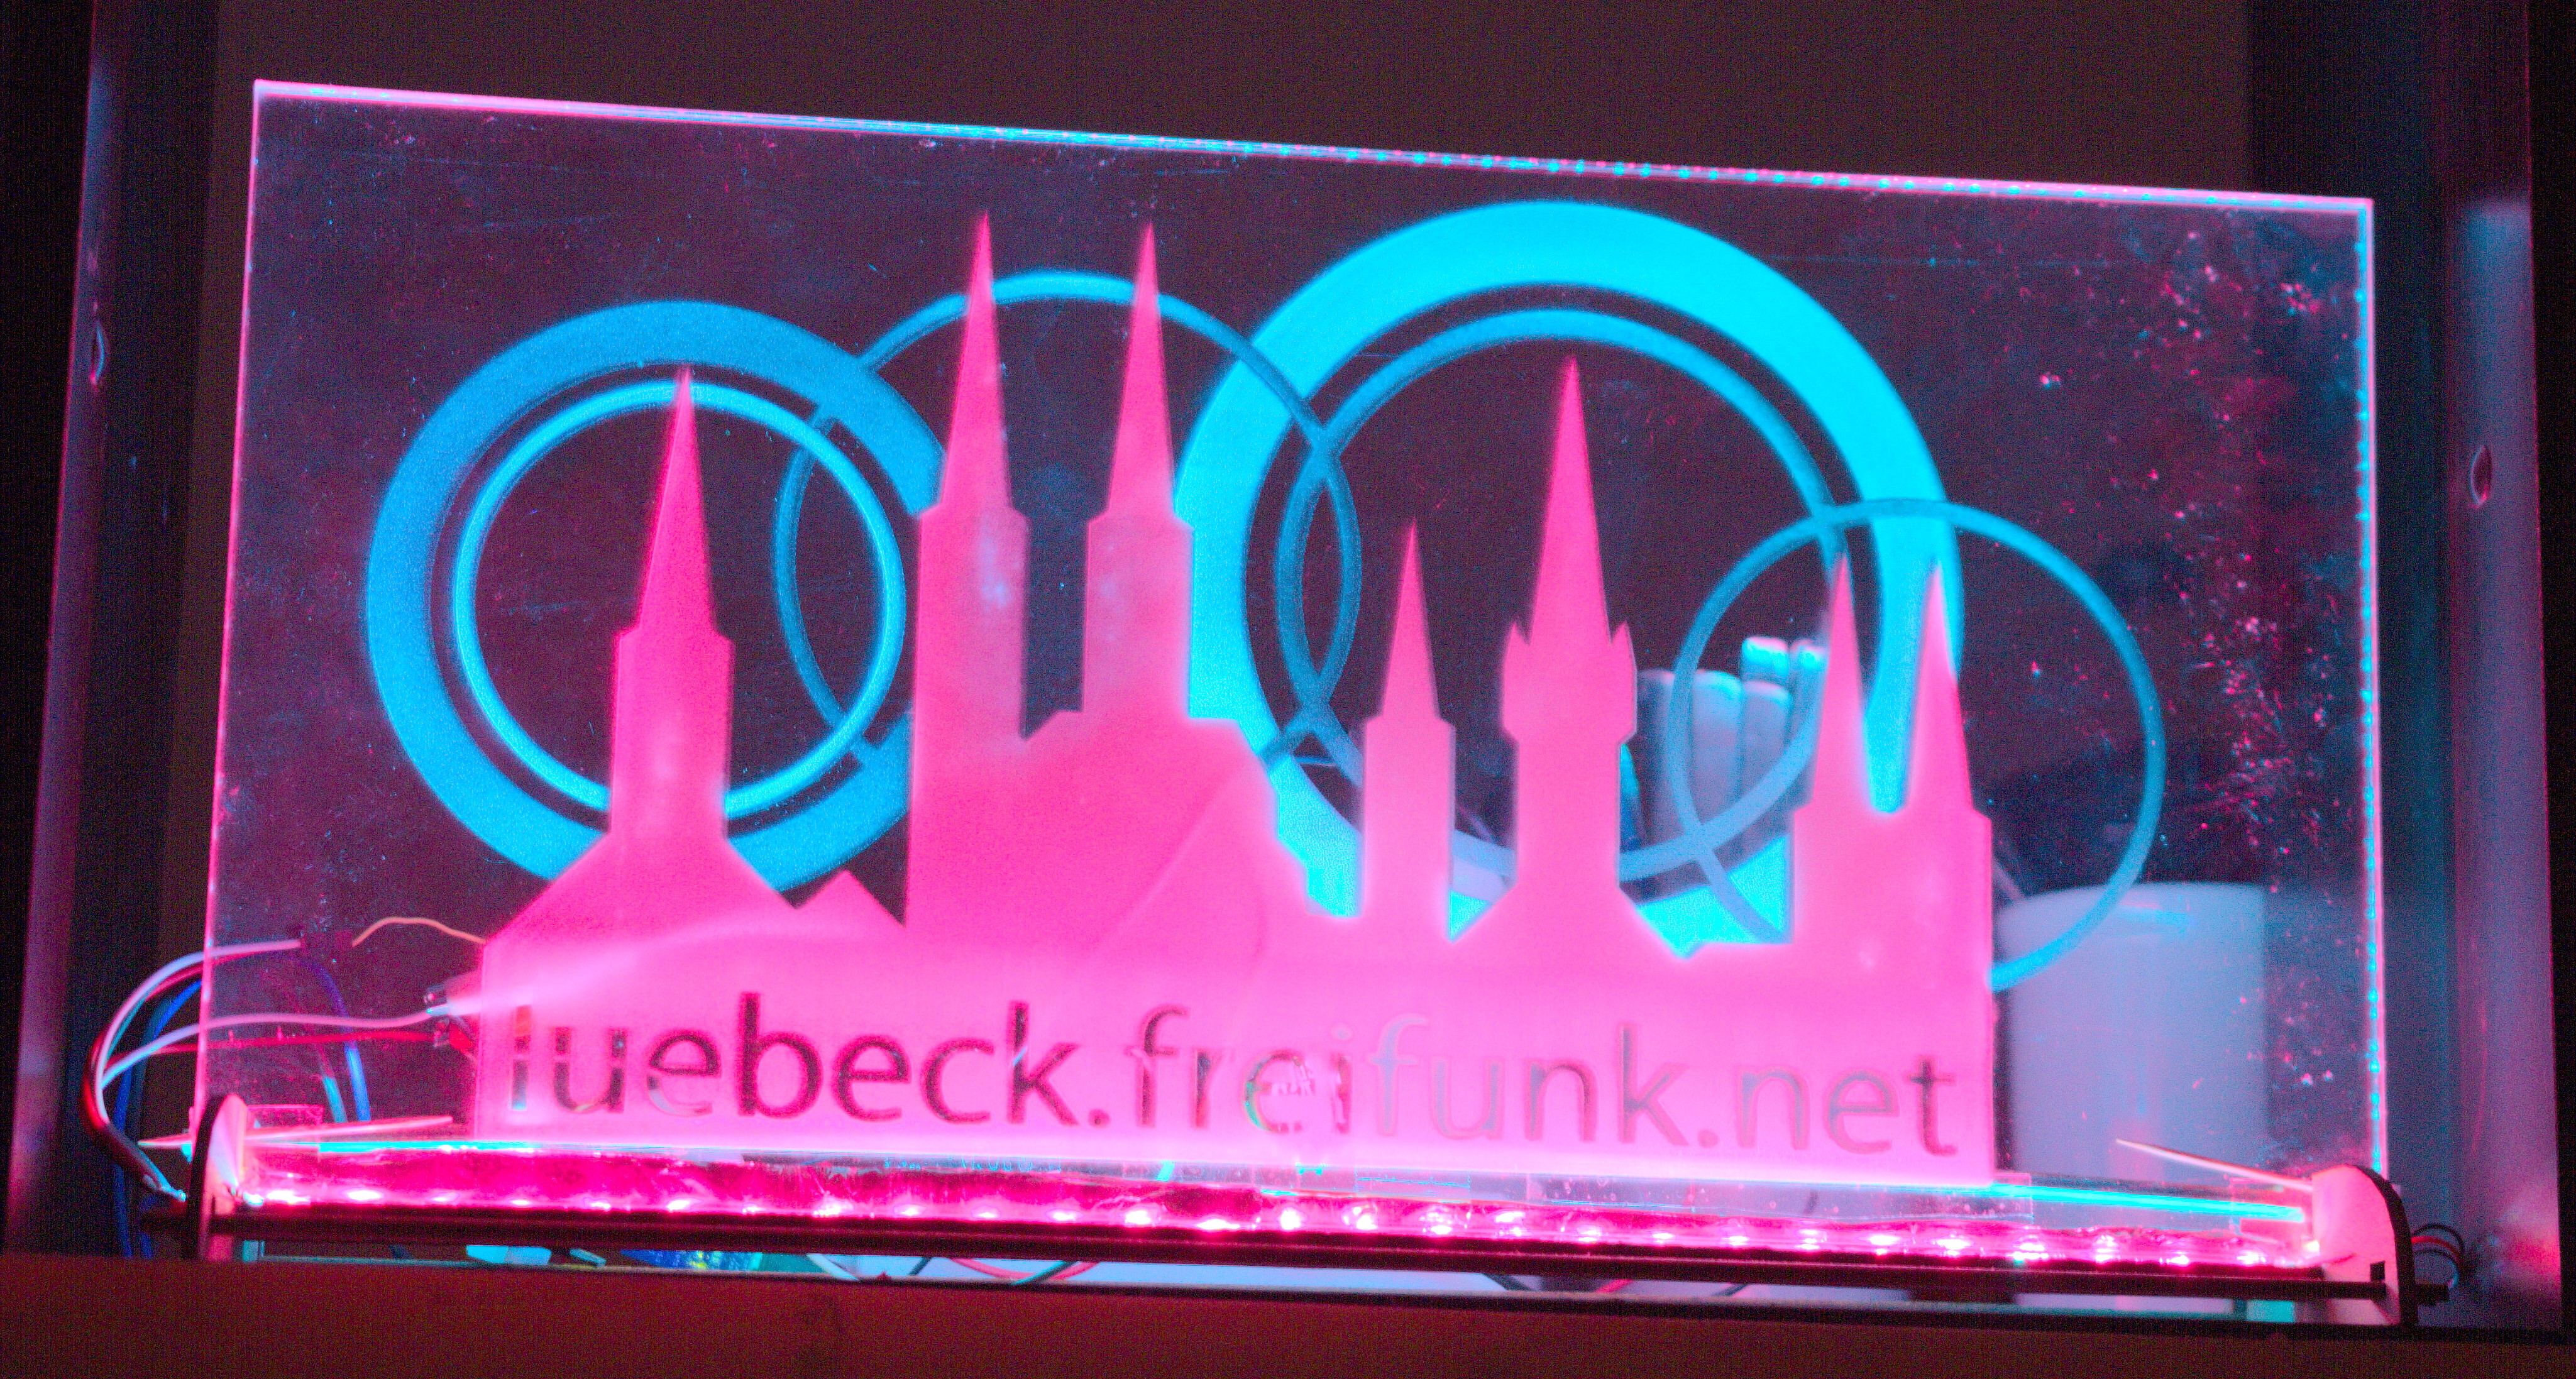
\includegraphics[width=12cm,keepaspectratio=true]{./img/_MGL5102.jpg}
\end{frame}

\subsection{Musik-Visualisierung}
\begin{frame}{Musik-Visualisierung}
\end{frame}

\subsection{Lichtquelle für ein Makroobjektiv}
\begin{frame}{Lichtquelle}
\centering
 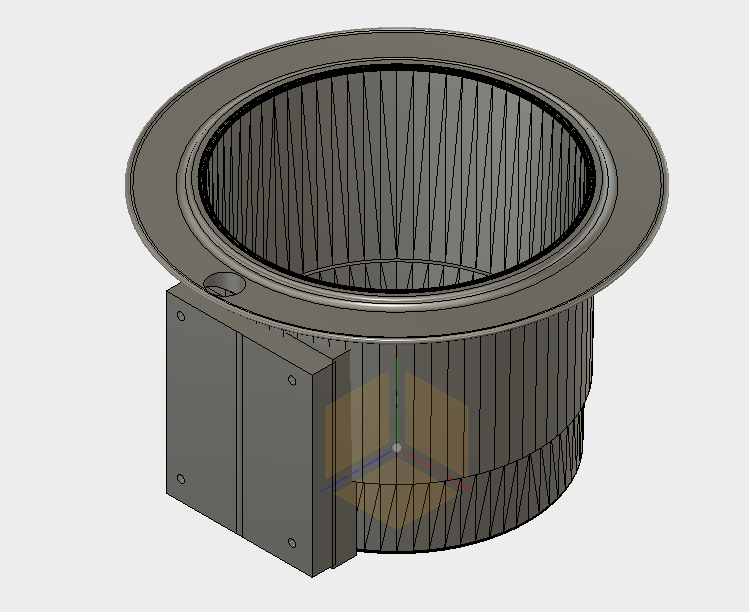
\includegraphics[width=6cm,keepaspectratio=true]{./img/screen.png}
\end{frame}

\section{Ressourcen}
\begin{frame}{Ressourcen}
 Hier Links zum git
\begin{itemize}
 \item \url{https://github.com/Gnoxter/Nook15-Vortrag}
 \item \url{https://github.com/Gnoxter/StripEvents}
 \item \url{https://github.com/adafruit/Adafruit_NeoPixel}
\end{itemize}
\end{frame}


\end{document}
